% Options for packages loaded elsewhere
\PassOptionsToPackage{unicode}{hyperref}
\PassOptionsToPackage{hyphens}{url}
%
\documentclass[
]{article}
\usepackage{lmodern}
\usepackage{amssymb,amsmath}
\usepackage{ifxetex,ifluatex}
\ifnum 0\ifxetex 1\fi\ifluatex 1\fi=0 % if pdftex
  \usepackage[T1]{fontenc}
  \usepackage[utf8]{inputenc}
  \usepackage{textcomp} % provide euro and other symbols
\else % if luatex or xetex
  \usepackage{unicode-math}
  \defaultfontfeatures{Scale=MatchLowercase}
  \defaultfontfeatures[\rmfamily]{Ligatures=TeX,Scale=1}
\fi
% Use upquote if available, for straight quotes in verbatim environments
\IfFileExists{upquote.sty}{\usepackage{upquote}}{}
\IfFileExists{microtype.sty}{% use microtype if available
  \usepackage[]{microtype}
  \UseMicrotypeSet[protrusion]{basicmath} % disable protrusion for tt fonts
}{}
\makeatletter
\@ifundefined{KOMAClassName}{% if non-KOMA class
  \IfFileExists{parskip.sty}{%
    \usepackage{parskip}
  }{% else
    \setlength{\parindent}{0pt}
    \setlength{\parskip}{6pt plus 2pt minus 1pt}}
}{% if KOMA class
  \KOMAoptions{parskip=half}}
\makeatother
\usepackage{xcolor}
\IfFileExists{xurl.sty}{\usepackage{xurl}}{} % add URL line breaks if available
\IfFileExists{bookmark.sty}{\usepackage{bookmark}}{\usepackage{hyperref}}
\hypersetup{
  pdftitle={753 - Problem Set 5},
  pdfauthor={Jesús Lara},
  hidelinks,
  pdfcreator={LaTeX via pandoc}}
\urlstyle{same} % disable monospaced font for URLs
\usepackage[margin=1in]{geometry}
\usepackage{color}
\usepackage{fancyvrb}
\newcommand{\VerbBar}{|}
\newcommand{\VERB}{\Verb[commandchars=\\\{\}]}
\DefineVerbatimEnvironment{Highlighting}{Verbatim}{commandchars=\\\{\}}
% Add ',fontsize=\small' for more characters per line
\usepackage{framed}
\definecolor{shadecolor}{RGB}{248,248,248}
\newenvironment{Shaded}{\begin{snugshade}}{\end{snugshade}}
\newcommand{\AlertTok}[1]{\textcolor[rgb]{0.94,0.16,0.16}{#1}}
\newcommand{\AnnotationTok}[1]{\textcolor[rgb]{0.56,0.35,0.01}{\textbf{\textit{#1}}}}
\newcommand{\AttributeTok}[1]{\textcolor[rgb]{0.77,0.63,0.00}{#1}}
\newcommand{\BaseNTok}[1]{\textcolor[rgb]{0.00,0.00,0.81}{#1}}
\newcommand{\BuiltInTok}[1]{#1}
\newcommand{\CharTok}[1]{\textcolor[rgb]{0.31,0.60,0.02}{#1}}
\newcommand{\CommentTok}[1]{\textcolor[rgb]{0.56,0.35,0.01}{\textit{#1}}}
\newcommand{\CommentVarTok}[1]{\textcolor[rgb]{0.56,0.35,0.01}{\textbf{\textit{#1}}}}
\newcommand{\ConstantTok}[1]{\textcolor[rgb]{0.00,0.00,0.00}{#1}}
\newcommand{\ControlFlowTok}[1]{\textcolor[rgb]{0.13,0.29,0.53}{\textbf{#1}}}
\newcommand{\DataTypeTok}[1]{\textcolor[rgb]{0.13,0.29,0.53}{#1}}
\newcommand{\DecValTok}[1]{\textcolor[rgb]{0.00,0.00,0.81}{#1}}
\newcommand{\DocumentationTok}[1]{\textcolor[rgb]{0.56,0.35,0.01}{\textbf{\textit{#1}}}}
\newcommand{\ErrorTok}[1]{\textcolor[rgb]{0.64,0.00,0.00}{\textbf{#1}}}
\newcommand{\ExtensionTok}[1]{#1}
\newcommand{\FloatTok}[1]{\textcolor[rgb]{0.00,0.00,0.81}{#1}}
\newcommand{\FunctionTok}[1]{\textcolor[rgb]{0.00,0.00,0.00}{#1}}
\newcommand{\ImportTok}[1]{#1}
\newcommand{\InformationTok}[1]{\textcolor[rgb]{0.56,0.35,0.01}{\textbf{\textit{#1}}}}
\newcommand{\KeywordTok}[1]{\textcolor[rgb]{0.13,0.29,0.53}{\textbf{#1}}}
\newcommand{\NormalTok}[1]{#1}
\newcommand{\OperatorTok}[1]{\textcolor[rgb]{0.81,0.36,0.00}{\textbf{#1}}}
\newcommand{\OtherTok}[1]{\textcolor[rgb]{0.56,0.35,0.01}{#1}}
\newcommand{\PreprocessorTok}[1]{\textcolor[rgb]{0.56,0.35,0.01}{\textit{#1}}}
\newcommand{\RegionMarkerTok}[1]{#1}
\newcommand{\SpecialCharTok}[1]{\textcolor[rgb]{0.00,0.00,0.00}{#1}}
\newcommand{\SpecialStringTok}[1]{\textcolor[rgb]{0.31,0.60,0.02}{#1}}
\newcommand{\StringTok}[1]{\textcolor[rgb]{0.31,0.60,0.02}{#1}}
\newcommand{\VariableTok}[1]{\textcolor[rgb]{0.00,0.00,0.00}{#1}}
\newcommand{\VerbatimStringTok}[1]{\textcolor[rgb]{0.31,0.60,0.02}{#1}}
\newcommand{\WarningTok}[1]{\textcolor[rgb]{0.56,0.35,0.01}{\textbf{\textit{#1}}}}
\usepackage{graphicx,grffile}
\makeatletter
\def\maxwidth{\ifdim\Gin@nat@width>\linewidth\linewidth\else\Gin@nat@width\fi}
\def\maxheight{\ifdim\Gin@nat@height>\textheight\textheight\else\Gin@nat@height\fi}
\makeatother
% Scale images if necessary, so that they will not overflow the page
% margins by default, and it is still possible to overwrite the defaults
% using explicit options in \includegraphics[width, height, ...]{}
\setkeys{Gin}{width=\maxwidth,height=\maxheight,keepaspectratio}
% Set default figure placement to htbp
\makeatletter
\def\fps@figure{htbp}
\makeatother
\setlength{\emergencystretch}{3em} % prevent overfull lines
\providecommand{\tightlist}{%
  \setlength{\itemsep}{0pt}\setlength{\parskip}{0pt}}
\setcounter{secnumdepth}{-\maxdimen} % remove section numbering
\usepackage{booktabs}
\usepackage{longtable}
\usepackage{array}
\usepackage{multirow}
\usepackage{wrapfig}
\usepackage{float}
\usepackage{colortbl}
\usepackage{pdflscape}
\usepackage{tabu}
\usepackage{threeparttable}
\usepackage{threeparttablex}
\usepackage[normalem]{ulem}
\usepackage{makecell}
\usepackage{xcolor}

\title{753 - Problem Set 5}
\author{Jesús Lara}
\date{11/17/2020}

\begin{document}
\maketitle

\hypertarget{granger-causality}{%
\section{Granger Causality}\label{granger-causality}}

In this exercise we work with time series of the Federal Funds and BAA
corporate yield rates to test the theory that Central Banks, through
open market operations, can determine or at least influence to an
important degree the market interest rate. We make use of the concept of
Granger causality: we test whether the lagged values of time series X
help to predict the current value of time-series Y.

The Granger causality procedure tests the null hypothesis that the
coefficients of the lagged values of time series X are jointly equal to
zero, so we need both time series to be stationary in order to avoid
spurious correlations. A time series is stationary if it has constant
mean, variance, and autocorrelation is the same for values at the same
distance in time. We plot the two rates in Figure 1. By visual
inspection, we can see that both follow trends: upward until 1982 and
downwards after that. This means that the means are not constant and
hence our series are very likely to be nonstationary.

\begin{figure}

{\centering 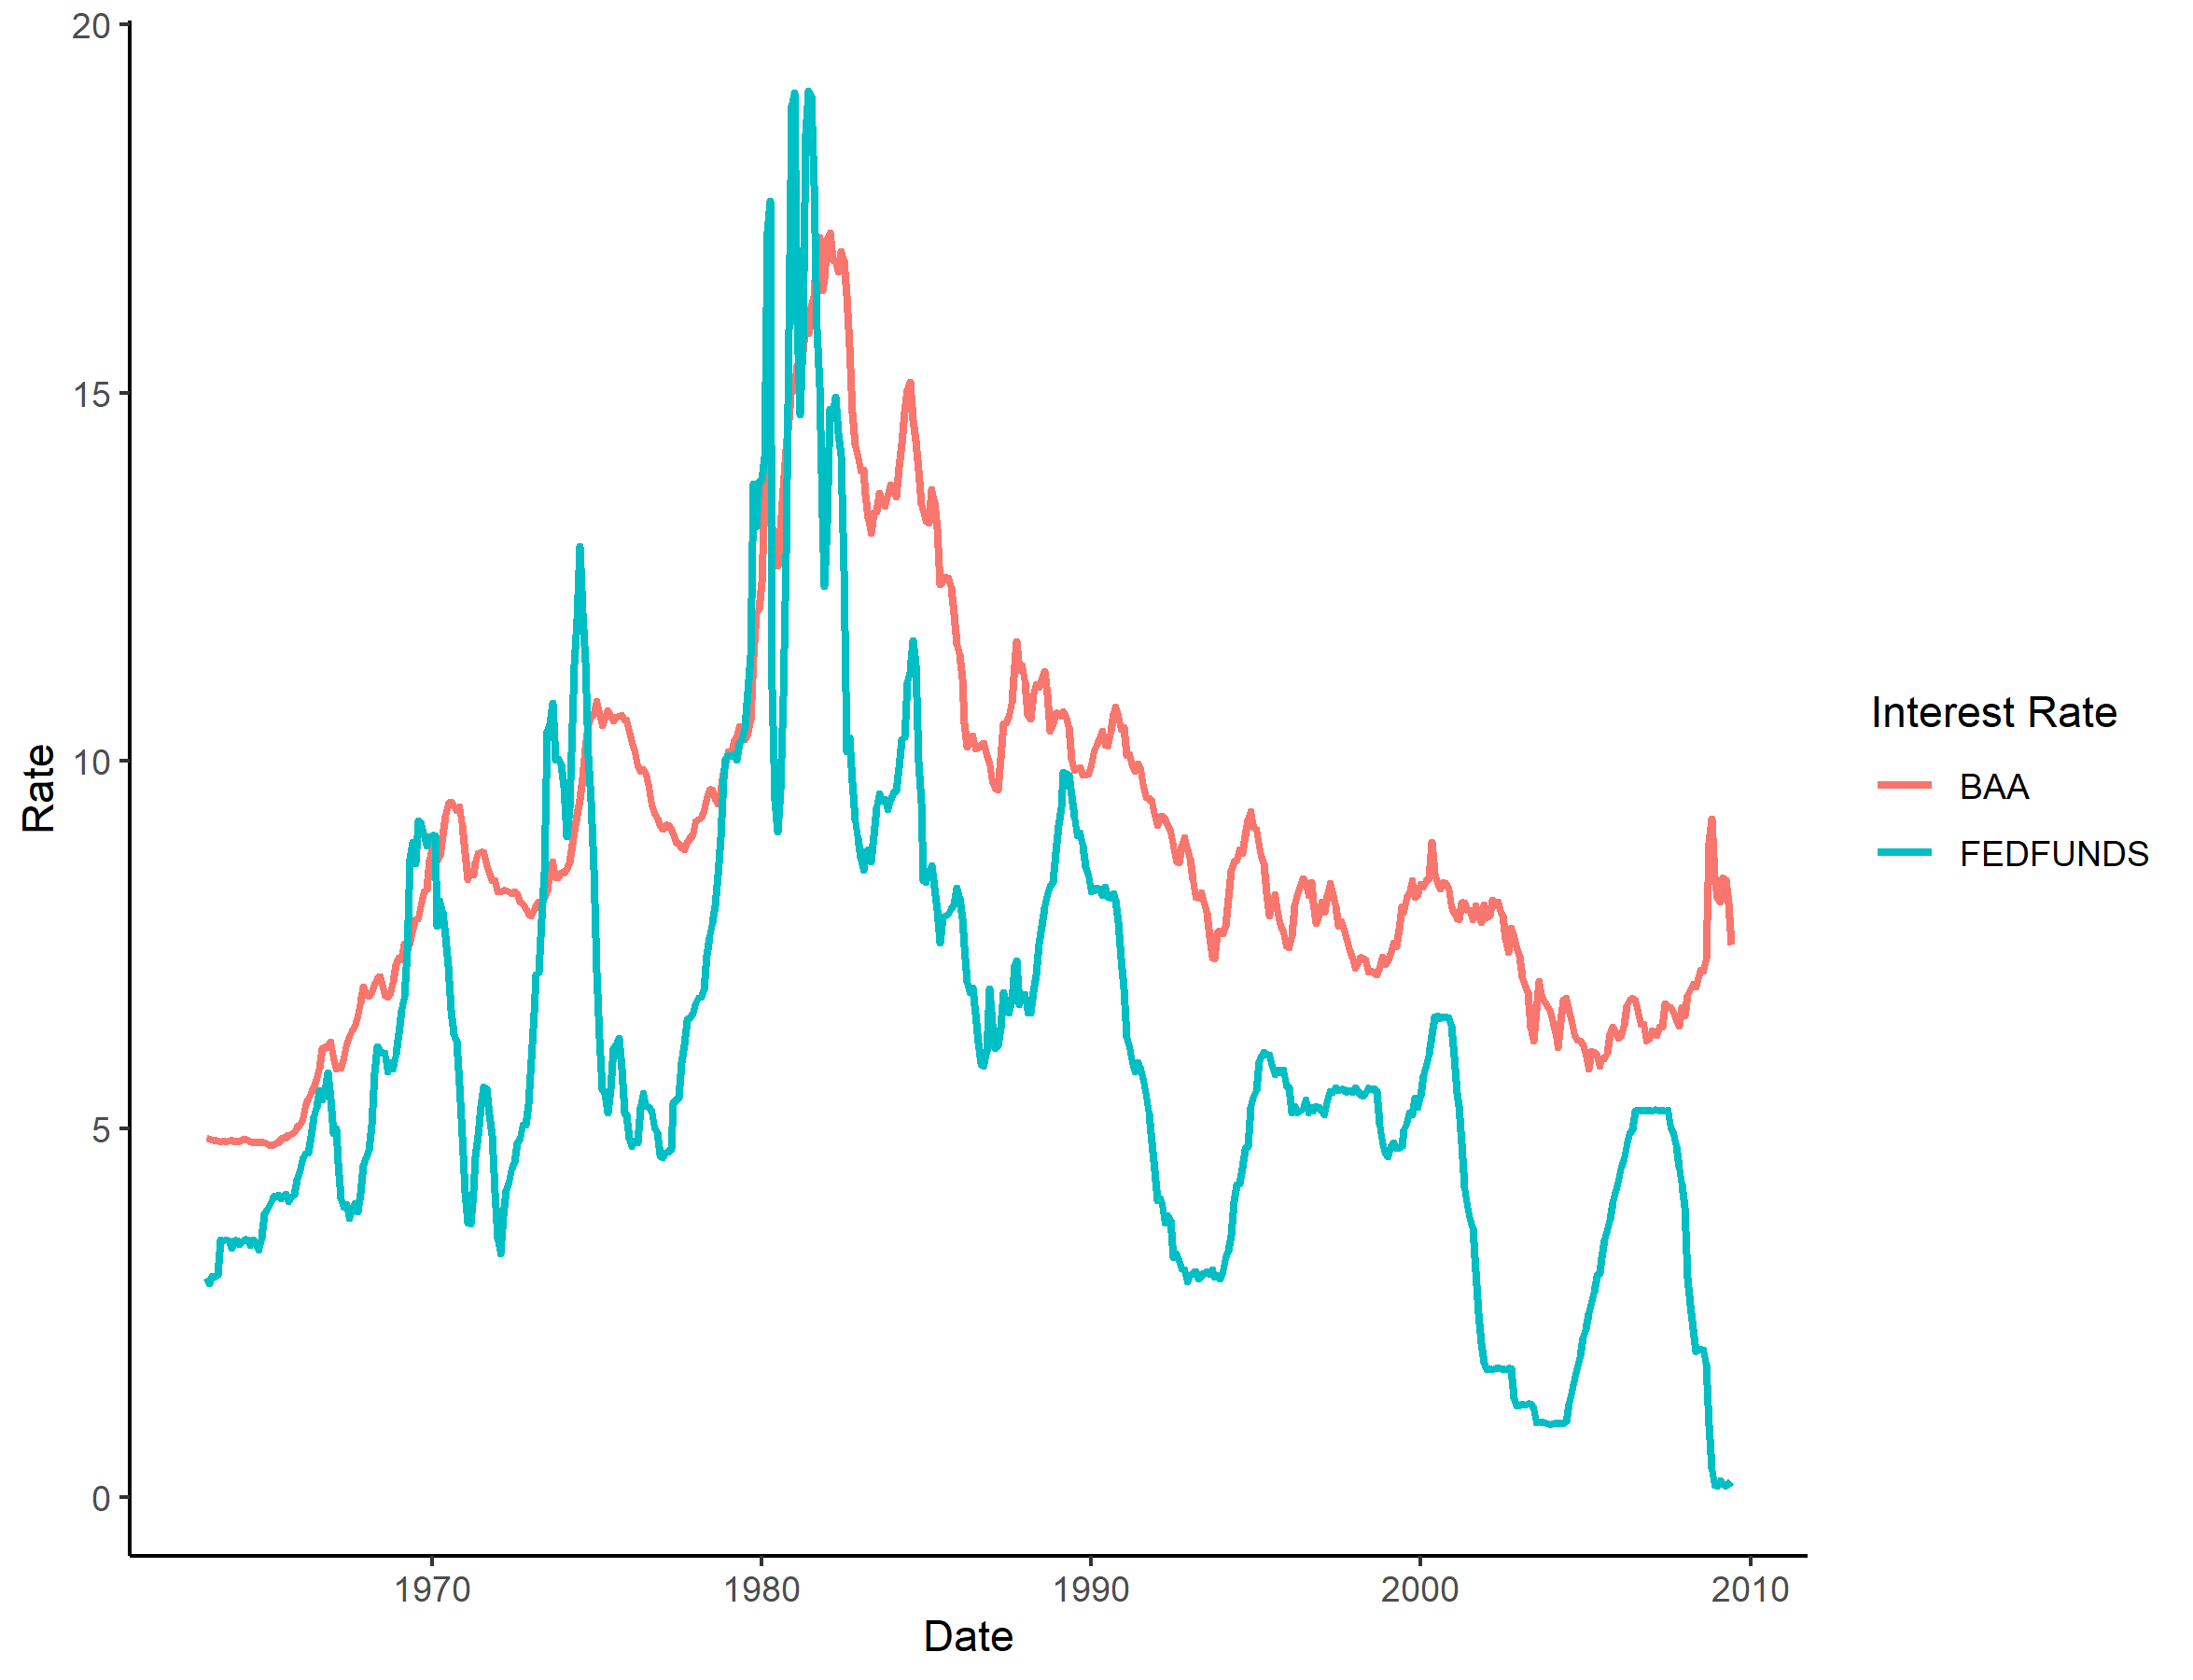
\includegraphics[width=0.75\linewidth]{BAA.FEDFUNDS.time.series} 

}

\caption{BAA and FED Funds rates time series}\label{fig:unnamed-chunk-2}
\end{figure}

Formally, a non-stationary time-series can be described by a random-walk
process:

\[y_t=y_{t-1}+v_t\]

The Augmented Dickey-Fuller (ADF) test tests whether the coefficient of
\(y_{t-1}\) is less or equal than one for three different
specifications:

Type 1: \(y_t=\rho y_{t-1}+v_t\) (No constant and no trend)

Type 2: \(y_t=\alpha + \rho y_{t-1}+v_t\) (With constant but no trend)

Type 3: \(y_t=\alpha + \rho y_{t-1} +\lambda t+v_t\) (With constant but
no trend)

The null hypothesis is \(H_0:\rho=1\) and the alternative is
\(H_1: \rho <1\). Hence, rejecting the null hypothesis is evidence in
favor of our time series being stationary. The test is augmented in the
sense that it controls for autocorrelarion of the error term by
including the number of lags of the time series such that the
autocorrelation becomes zero. The results are presented in Table 1. By
looking at the p-values, we can see that we fail to reject the null
hypothesis at any reasonable level of significance. Hence, we conclude
that our time series are non-stationary.

\begin{table}

\caption{\label{tab:unnamed-chunk-3}Augmented Dickey-Fuller Test}
\centering
\resizebox{\linewidth}{!}{
\begin{tabular}[t]{rrrrrrrrrrrrr}
\toprule
\multicolumn{1}{c}{ } & \multicolumn{6}{c}{BAA} & \multicolumn{6}{c}{FEDFUNDS} \\
\cmidrule(l{3pt}r{3pt}){2-7} \cmidrule(l{3pt}r{3pt}){8-13}
\multicolumn{1}{c}{ } & \multicolumn{2}{c}{Type 1} & \multicolumn{2}{c}{Type 2} & \multicolumn{2}{c}{Type 3} & \multicolumn{2}{c}{Type 1} & \multicolumn{2}{c}{Type 2} & \multicolumn{2}{c}{Type 3} \\
\cmidrule(l{3pt}r{3pt}){2-3} \cmidrule(l{3pt}r{3pt}){4-5} \cmidrule(l{3pt}r{3pt}){6-7} \cmidrule(l{3pt}r{3pt}){8-9} \cmidrule(l{3pt}r{3pt}){10-11} \cmidrule(l{3pt}r{3pt}){12-13}
Lag & ADF & P-Value & ADF & P-Value & ADF & P-Value & ADF & P-Value & ADF & P-Value & ADF & P-Value\\
\midrule
0 & 0.034 & 0.654 & -1.507 & 0.522 & -1.612 & 0.742 & -1.015 & 0.316 & -1.761 & 0.423 & -2.242 & 0.474\\
1 & -0.274 & 0.565 & -1.861 & 0.384 & -1.940 & 0.602 & -1.513 & 0.138 & -2.983 & 0.039 & -3.404 & 0.053\\
2 & -0.140 & 0.604 & -1.690 & 0.452 & -1.786 & 0.668 & -1.278 & 0.222 & -2.426 & 0.158 & -2.865 & 0.211\\
3 & -0.181 & 0.592 & -1.745 & 0.430 & -1.842 & 0.644 & -1.225 & 0.241 & -2.326 & 0.198 & -2.781 & 0.247\\
4 & -0.230 & 0.578 & -1.824 & 0.399 & -1.920 & 0.611 & -1.143 & 0.270 & -2.129 & 0.277 & -2.600 & 0.323\\
\addlinespace
5 & -0.261 & 0.569 & -1.881 & 0.376 & -1.979 & 0.586 & -1.158 & 0.265 & -2.102 & 0.287 & -2.554 & 0.343\\
\bottomrule
\end{tabular}}
\end{table}

In Figure 2 we show the first-differences of our time
series(\(\Delta y_t=y_t-y_{t-1}\)) . We can see that all fluctuations
occur around 0, although the magnitude of these fluctuations vary
between periods: before 1982 and after 1982. The results of the ADF test
for the differenced time series are presented in Table 2.

\begin{figure}

{\centering 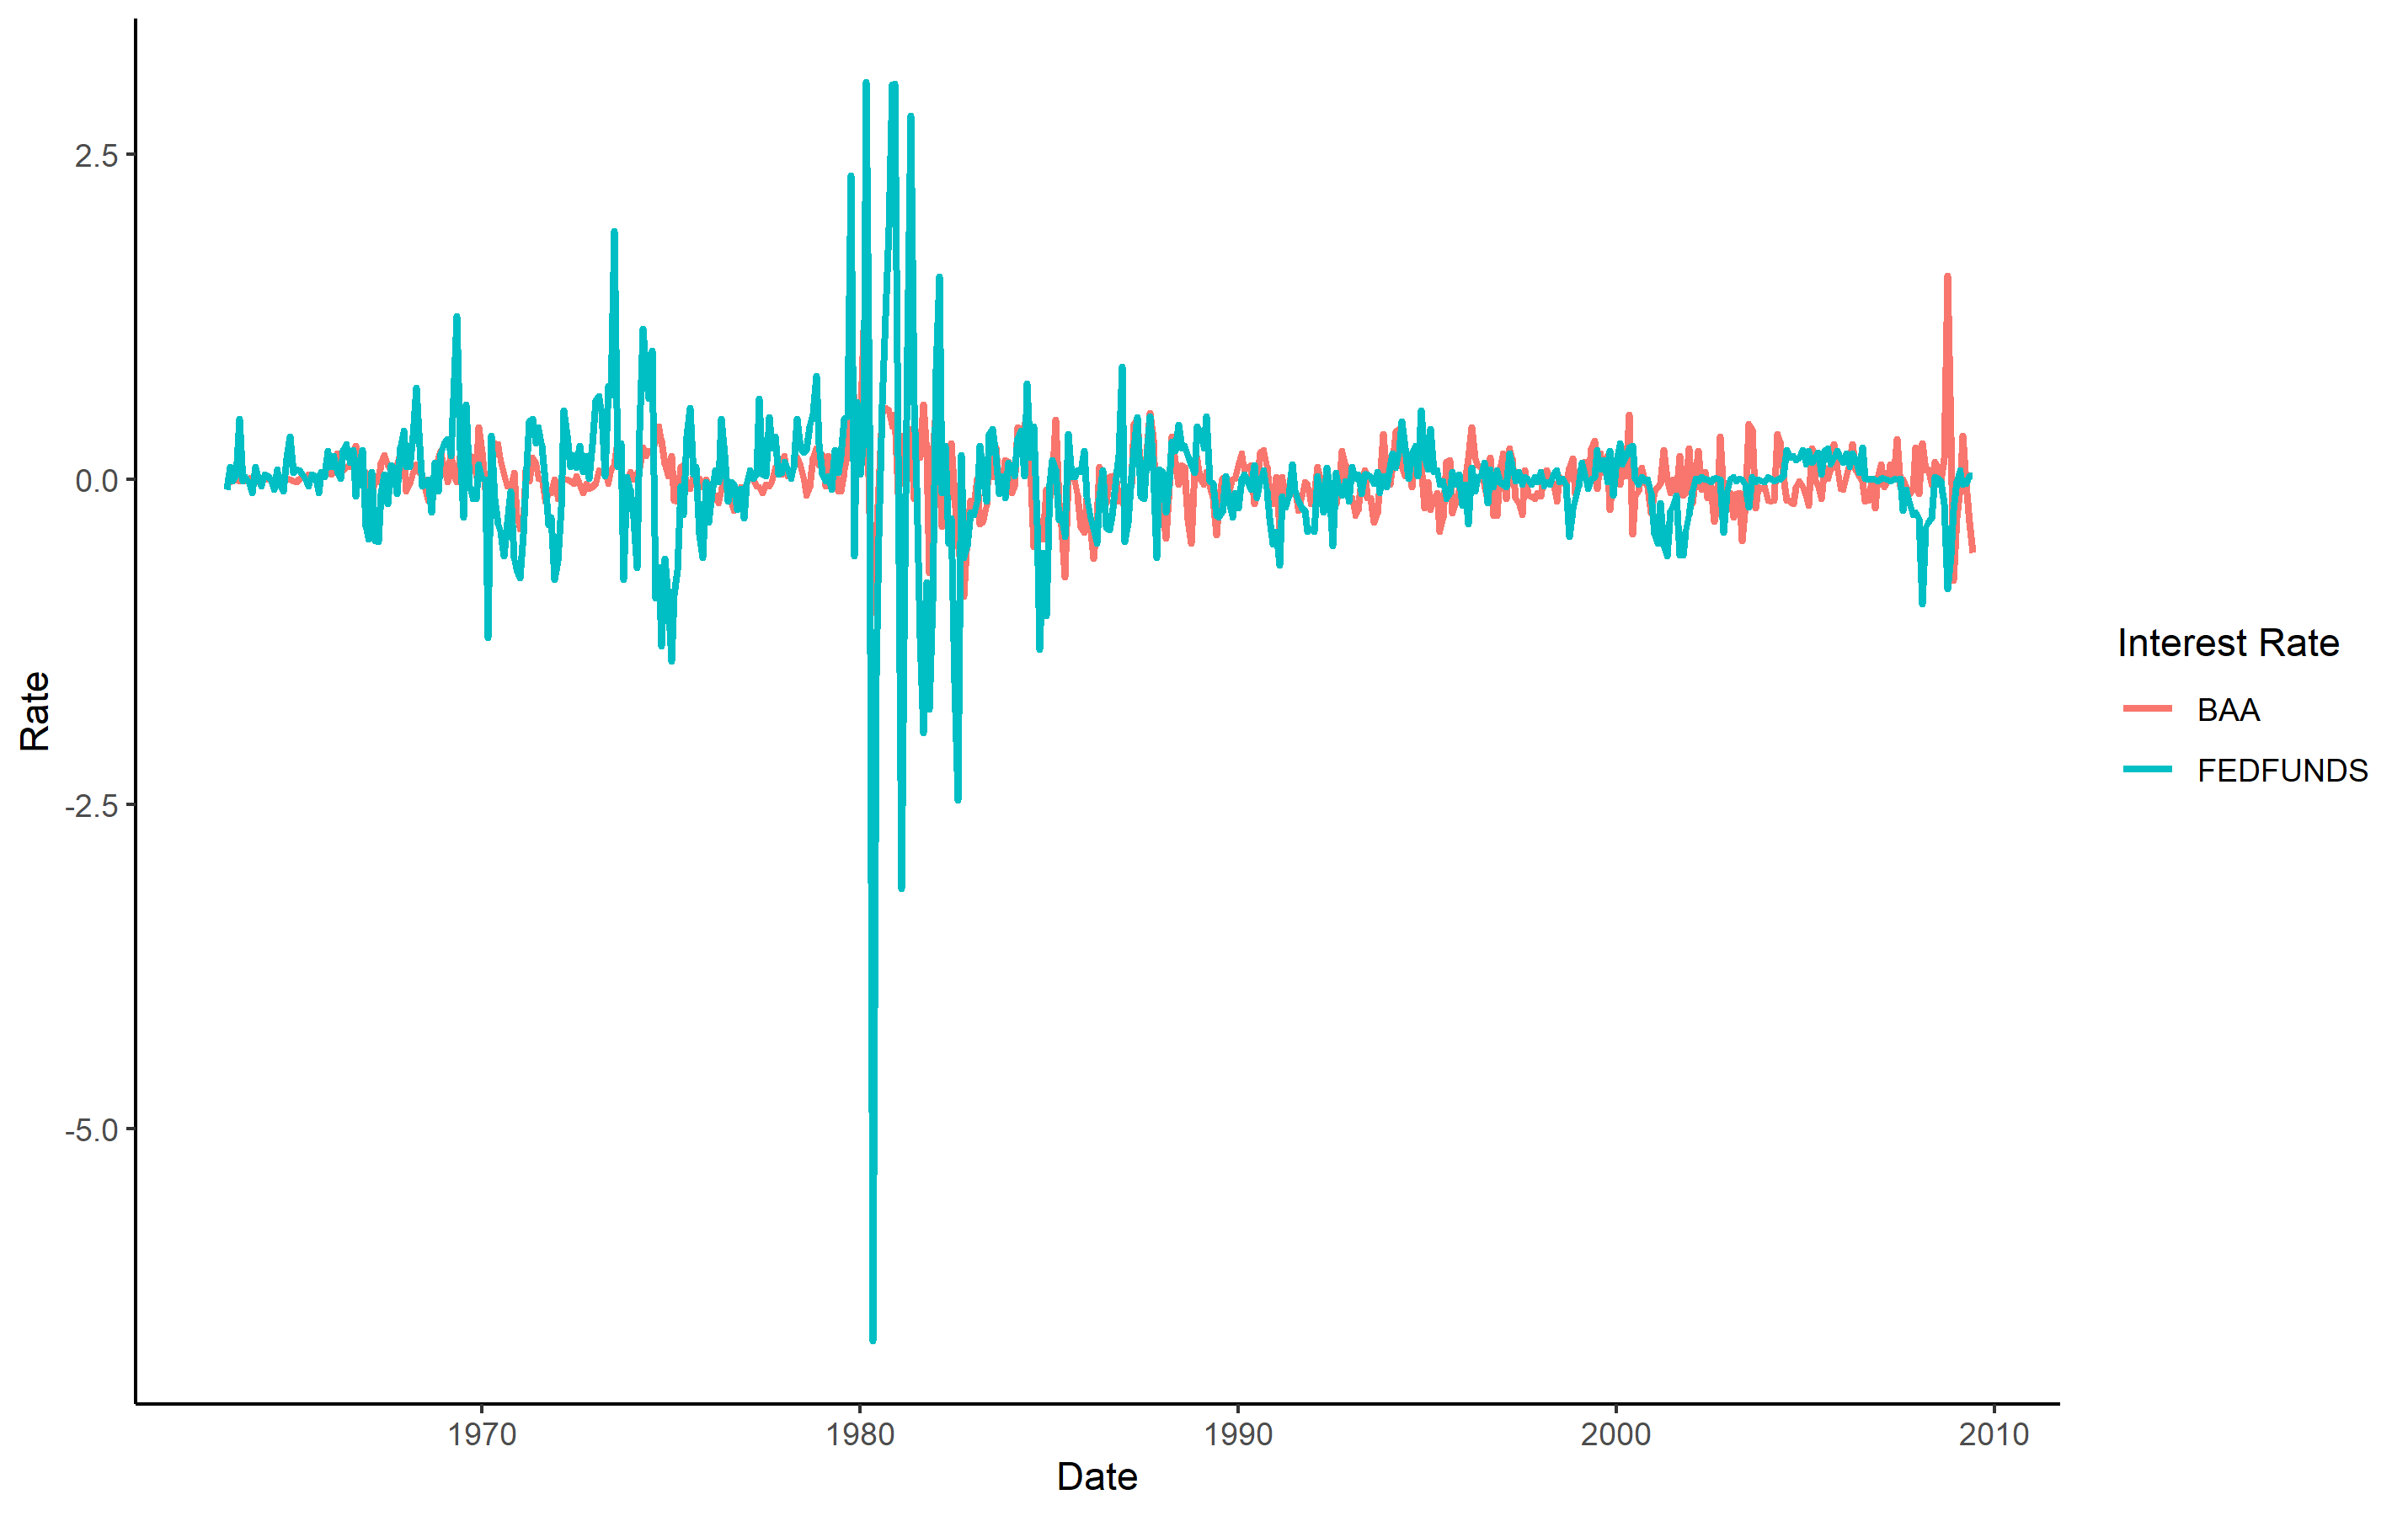
\includegraphics[width=0.75\linewidth]{BAA.FEDFUNDS.d.time.series} 

}

\caption{BAA and FED Funds rates time series. (First differences)}\label{fig:unnamed-chunk-4}
\end{figure}

\begin{table}

\caption{\label{tab:unnamed-chunk-5}Augmented Dickey-Fuller Test: First difference of rates}
\centering
\resizebox{\linewidth}{!}{
\begin{tabular}[t]{rrrrrrrrrrrrr}
\toprule
\multicolumn{1}{c}{ } & \multicolumn{6}{c}{BAA} & \multicolumn{6}{c}{FEDFUNDS} \\
\cmidrule(l{3pt}r{3pt}){2-7} \cmidrule(l{3pt}r{3pt}){8-13}
\multicolumn{1}{c}{ } & \multicolumn{2}{c}{Type 1} & \multicolumn{2}{c}{Type 2} & \multicolumn{2}{c}{Type 3} & \multicolumn{2}{c}{Type 1} & \multicolumn{2}{c}{Type 2} & \multicolumn{2}{c}{Type 3} \\
\cmidrule(l{3pt}r{3pt}){2-3} \cmidrule(l{3pt}r{3pt}){4-5} \cmidrule(l{3pt}r{3pt}){6-7} \cmidrule(l{3pt}r{3pt}){8-9} \cmidrule(l{3pt}r{3pt}){10-11} \cmidrule(l{3pt}r{3pt}){12-13}
Lag & ADF & P-Value & ADF & P-Value & ADF & P-Value & ADF & P-Value & ADF & P-Value & ADF & P-Value\\
\midrule
0 & -15.086 & 0.01 & -15.075 & 0.01 & -15.131 & 0.01 & -15.339 & 0.01 & -15.326 & 0.01 & -15.339 & 0.01\\
1 & -15.104 & 0.01 & -15.096 & 0.01 & -15.176 & 0.01 & -15.369 & 0.01 & -15.356 & 0.01 & -15.380 & 0.01\\
2 & -11.928 & 0.01 & -11.922 & 0.01 & -12.008 & 0.01 & -13.389 & 0.01 & -13.378 & 0.01 & -13.411 & 0.01\\
3 & -9.859 & 0.01 & -9.855 & 0.01 & -9.942 & 0.01 & -12.511 & 0.01 & -12.501 & 0.01 & -12.544 & 0.01\\
4 & -8.664 & 0.01 & -8.660 & 0.01 & -8.752 & 0.01 & -11.029 & 0.01 & -11.022 & 0.01 & -11.062 & 0.01\\
\addlinespace
5 & -8.021 & 0.01 & -8.018 & 0.01 & -8.114 & 0.01 & -10.551 & 0.01 & -10.544 & 0.01 & -10.598 & 0.01\\
\bottomrule
\end{tabular}}
\end{table}

The null-hypothesis is rejected at the 1\% level of significance. So we
can conclude that the differenced time series are stationary. Now we
conduct the Granger causality tests in both directions: The BAA rate
Granger causes the FED Funds Rate and the other way round. For the test
we include three different specifications: 2, 5 and 10 lags. The results
for the whole period are shown in the first two columns of Table 2. We
reject the null hypothesis that the BAA rate does not Granger Cause the
FED Funds rate at all levels of statistical signficance. In contrast, we
fail to reject the null that the Fed Funds Rate does not Granger cause
the BAA rate. Hence, our results go against the theory of the exogeneity
of the interest rate: not only the FED funds rate does not precede and
predicts the BAA rate, but it actually happens the opposite way.

For robustness, we perform the same test but for two separate periods:
before and after 19882 as, by Figure 1, we can observe that in that year
both rates reached their maximum and after that they started to decline.
This may be associated to the debt crisis that exploded first in Mexico
and then in Latin America after the sharp increase in the interest rates
in 1981. The results are presented in columns 3 to 6 of Table 3. For the
first period, our basic result that the BAA rate causes the FED Funds
rate but not the other way round remains. However, we see that for the
specification with 10 lags, the FED Funds rate actually Granger causes
the BAA rate. However, when we consider only the (1982-02)-(2009-06)
periods, our results show that the BAA rate does not longer Granger
causes the FED Funds Rate. Actually, it seems that in this recent
period, the FED Funds Rate weakly granger causes the BAA rate in the
very short-run, as the only specification which is statistically
significant at the 5\% level is the one with only two lags.

The conclusion of this analysis is that we do not have statistical
evidence in favor of interest rate exogeneity, which is one of the core
elements of mainstream macroeconomic theory.

\begin{table}

\caption{\label{tab:unnamed-chunk-6}Granger Causality Tests: BAA and FEDFUNDS}
\centering
\begin{tabular}[t]{rrrrrrr}
\toprule
\multicolumn{1}{c}{} & \multicolumn{2}{c}{(1961-03)-(2009-06)} & \multicolumn{2}{c}{(1961-03)-(1982-01)} & \multicolumn{2}{c}{(1982-02)-(2009-06)} \\
\cmidrule(l{3pt}r{3pt}){2-3} \cmidrule(l{3pt}r{3pt}){4-5} \cmidrule(l{3pt}r{3pt}){6-7}
Lags & F & P-Value & F & P-Value & F & P-Value\\
\midrule
\addlinespace[0.3em]
\multicolumn{7}{l}{\textbf{BAA Rate Granger causes FED Funds Rate}}\\
\hspace{1em}2 & 8.766 & 0.000 & 12.854 & 0.000 & 0.411 & 0.663\\
\hspace{1em}5 & 3.709 & 0.003 & 5.748 & 0.000 & 0.596 & 0.703\\
\hspace{1em}10 & 4.270 & 0.000 & 9.675 & 0.000 & 0.939 & 0.497\\
\addlinespace[0.3em]
\multicolumn{7}{l}{\textbf{FED Funds Rate Granger causes BAA Rate}}\\
\hspace{1em}2 & 1.658 & 0.191 & 0.107 & 0.898 & 3.857 & 0.022\\
\hspace{1em}5 & 1.716 & 0.129 & 1.252 & 0.286 & 1.925 & 0.090\\
\hspace{1em}10 & 1.944 & 0.037 & 3.100 & 0.001 & 0.496 & 0.892\\
\bottomrule
\end{tabular}
\end{table}

\hypertarget{replication}{%
\section{Replication}\label{replication}}

I presented my advances in the previous problem set. They consist of
tables of summary statistics of the main variables: Rules of Origin,
Tariffs and Imports at the product level (6 digits according to the
Harmonized System). I obtained the data from the online supplemental
material of the AEA. In order to exactly replicate their results, I am
following step by step their Stata code (I am working in R). However, I
have identified some weird steps and one of my extensions would be to
work with the Raw data as it is, constructing the variables just as they
are defined and then compare my results with those of the original
paper.

\pagebreak

\hypertarget{r-code}{%
\section{R code}\label{r-code}}

\begin{Shaded}
\begin{Highlighting}[]
\CommentTok{#Econ 753}
\CommentTok{#PS5}
\CommentTok{#Jesús Lara}

\KeywordTok{library}\NormalTok{(dplyr)}
\KeywordTok{library}\NormalTok{(tidyr)}
\KeywordTok{library}\NormalTok{(data.table)}
\KeywordTok{library}\NormalTok{(ggplot2)}
\KeywordTok{library}\NormalTok{(}\StringTok{"rio"}\NormalTok{)}
\KeywordTok{library}\NormalTok{(matlib)}
\KeywordTok{library}\NormalTok{(gdata)}
\KeywordTok{library}\NormalTok{(tinytex)}
\KeywordTok{library}\NormalTok{(car)}
\KeywordTok{library}\NormalTok{(scales)}
\KeywordTok{library}\NormalTok{(ggplot2)}
\KeywordTok{library}\NormalTok{(foreign)}
\KeywordTok{library}\NormalTok{(rmarkdown)}
\KeywordTok{library}\NormalTok{(fastDummies)}
\KeywordTok{library}\NormalTok{(haven)}
\KeywordTok{library}\NormalTok{(pmdplyr)}
\KeywordTok{library}\NormalTok{(plotrix)}
\KeywordTok{library}\NormalTok{(foreign)}
\KeywordTok{library}\NormalTok{(stringr)}
\KeywordTok{library}\NormalTok{(alfred)}
\KeywordTok{library}\NormalTok{(aTSA)}
\KeywordTok{library}\NormalTok{(lmtest)  }\CommentTok{## For Granger causality}


\KeywordTok{options}\NormalTok{(}\DataTypeTok{scipen=}\DecValTok{10000}\NormalTok{)}
\KeywordTok{options}\NormalTok{(}\DataTypeTok{digits=}\DecValTok{4}\NormalTok{)}

\KeywordTok{rm}\NormalTok{(}\DataTypeTok{list=}\KeywordTok{ls}\NormalTok{())}

\KeywordTok{setwd}\NormalTok{(}\StringTok{"C:/Users/User/Documents/GitHub/Problem-Sets--753/PS5"}\NormalTok{)}

\CommentTok{### Part 2}

\NormalTok{BAA  <-}\StringTok{ }\KeywordTok{get_fred_series}\NormalTok{(}\StringTok{"BAA"}\NormalTok{, }\DataTypeTok{series_name=}\StringTok{"BAA"}\NormalTok{)   }
\NormalTok{FEDFUNDS  <-}\StringTok{ }\KeywordTok{get_fred_series}\NormalTok{(}\StringTok{"FEDFUNDS"}\NormalTok{, }\DataTypeTok{series_name=}\StringTok{"FEDFUNDS"}\NormalTok{) }


\KeywordTok{ggplot}\NormalTok{(BAA, }\KeywordTok{aes}\NormalTok{(}\DataTypeTok{x=}\NormalTok{date,}\DataTypeTok{y=}\NormalTok{BAA))}\OperatorTok{+}\KeywordTok{geom_line}\NormalTok{()}

\KeywordTok{ggplot}\NormalTok{(FEDFUNDS, }\KeywordTok{aes}\NormalTok{(}\DataTypeTok{x=}\NormalTok{date,}\DataTypeTok{y=}\NormalTok{FEDFUNDS))}\OperatorTok{+}\KeywordTok{geom_line}\NormalTok{()}

\CommentTok{#1}
\NormalTok{series<-}\KeywordTok{merge}\NormalTok{(BAA, FEDFUNDS, }\DataTypeTok{by=}\StringTok{"date"}\NormalTok{)}
\NormalTok{series<-series }\OperatorTok\StringTok{ }\KeywordTok{filter}\NormalTok{(date}\OperatorTok{>=}\StringTok{"1963-03-01"} \OperatorTok{&}\StringTok{ }\NormalTok{date}\OperatorTok{<=}\StringTok{"2009-06-01"}\NormalTok{)}

\KeywordTok{ggplot}\NormalTok{(series, }\KeywordTok{aes}\NormalTok{(}\DataTypeTok{x=}\NormalTok{date))}\OperatorTok{+}\KeywordTok{theme_classic}\NormalTok{() }\OperatorTok{+}\StringTok{ }
\StringTok{  }\KeywordTok{geom_line}\NormalTok{(}\KeywordTok{aes}\NormalTok{(}\DataTypeTok{y=}\NormalTok{BAA,}\DataTypeTok{color=}\StringTok{"black"}\NormalTok{),}\DataTypeTok{size=}\DecValTok{1}\NormalTok{)}\OperatorTok{+}
\StringTok{  }\KeywordTok{geom_line}\NormalTok{(}\KeywordTok{aes}\NormalTok{(}\DataTypeTok{y=}\NormalTok{FEDFUNDS,}\DataTypeTok{color=}\StringTok{"blue"}\NormalTok{),}\DataTypeTok{size=}\DecValTok{1}\NormalTok{)}\OperatorTok{+}
\StringTok{  }\KeywordTok{xlab}\NormalTok{(}\StringTok{"Date"}\NormalTok{)}\OperatorTok{+}
\StringTok{  }\KeywordTok{ylab}\NormalTok{(}\StringTok{"Rate"}\NormalTok{)}\OperatorTok{+}
\StringTok{  }\KeywordTok{scale_color_discrete}\NormalTok{(}\DataTypeTok{name=}\StringTok{"Interest Rate"}\NormalTok{, }\DataTypeTok{label=}\KeywordTok{c}\NormalTok{(}\StringTok{"BAA"}\NormalTok{,}\StringTok{"FEDFUNDS"}\NormalTok{))}

\KeywordTok{ggsave}\NormalTok{(}\StringTok{"BAA.FEDFUNDS.time.series.png"}\NormalTok{)}


\NormalTok{BAA1<-}\KeywordTok{adf.test}\NormalTok{(series}\OperatorTok{$}\NormalTok{BAA)}
\NormalTok{FEDFUNDS1<-}\KeywordTok{adf.test}\NormalTok{(series}\OperatorTok{$}\NormalTok{FEDFUNDS)}


\CommentTok{## Create a Data Frame with results:}

\NormalTok{ADF1<-}\KeywordTok{data.frame}\NormalTok{(BAA1}\OperatorTok{$}\NormalTok{type1,BAA1}\OperatorTok{$}\NormalTok{type2[,}\DecValTok{2}\OperatorTok{:}\DecValTok{3}\NormalTok{],}
\NormalTok{                 BAA1}\OperatorTok{$}\NormalTok{type3[,}\DecValTok{2}\OperatorTok{:}\DecValTok{3}\NormalTok{],FEDFUNDS1}\OperatorTok{$}\NormalTok{type1[,}\DecValTok{2}\OperatorTok{:}\DecValTok{3}\NormalTok{], }
\NormalTok{                 FEDFUNDS1}\OperatorTok{$}\NormalTok{type2[,}\DecValTok{2}\OperatorTok{:}\DecValTok{3}\NormalTok{], FEDFUNDS1}\OperatorTok{$}\NormalTok{type3[,}\DecValTok{2}\OperatorTok{:}\DecValTok{3}\NormalTok{])}
\KeywordTok{colnames}\NormalTok{(ADF1)<-}\KeywordTok{c}\NormalTok{(}\StringTok{"Lag"}\NormalTok{,}\KeywordTok{rep}\NormalTok{(}\KeywordTok{c}\NormalTok{(}\StringTok{"ADF"}\NormalTok{, }\StringTok{"P-Value"}\NormalTok{),}\DecValTok{6}\NormalTok{))}
\KeywordTok{save}\NormalTok{(ADF1, }\DataTypeTok{file=}\StringTok{"ADF1.Rdata"}\NormalTok{)}

\CommentTok{#The series are non-stationary :(}


\CommentTok{#2 First difference data}


\NormalTok{series<-series }\OperatorTok\StringTok{ }\KeywordTok{mutate}\NormalTok{(}\DataTypeTok{d.BAA=}\KeywordTok{c}\NormalTok{(}\OtherTok{NA}\NormalTok{,}\KeywordTok{diff}\NormalTok{(BAA)),}
                          \DataTypeTok{d.FEDFUNDS=}\KeywordTok{c}\NormalTok{(}\OtherTok{NA}\NormalTok{,}\KeywordTok{diff}\NormalTok{(FEDFUNDS))) }\CommentTok{#Chulada}

\CommentTok{#Plot of differents}
\KeywordTok{ggplot}\NormalTok{(series, }\KeywordTok{aes}\NormalTok{(}\DataTypeTok{x=}\NormalTok{date), }\DataTypeTok{na.rm=}\OtherTok{TRUE}\NormalTok{)}\OperatorTok{+}\KeywordTok{theme_classic}\NormalTok{() }\OperatorTok{+}\StringTok{ }
\StringTok{  }\KeywordTok{geom_line}\NormalTok{(}\KeywordTok{aes}\NormalTok{(}\DataTypeTok{y=}\NormalTok{d.BAA,}\DataTypeTok{color=}\StringTok{"black"}\NormalTok{),}\DataTypeTok{size=}\DecValTok{1}\NormalTok{)}\OperatorTok{+}
\StringTok{  }\KeywordTok{geom_line}\NormalTok{(}\KeywordTok{aes}\NormalTok{(}\DataTypeTok{y=}\NormalTok{d.FEDFUNDS,}\DataTypeTok{color=}\StringTok{"blue"}\NormalTok{),}\DataTypeTok{size=}\DecValTok{1}\NormalTok{)}\OperatorTok{+}
\StringTok{  }\KeywordTok{xlab}\NormalTok{(}\StringTok{"Date"}\NormalTok{)}\OperatorTok{+}
\StringTok{  }\KeywordTok{ylab}\NormalTok{(}\StringTok{"Rate"}\NormalTok{)}\OperatorTok{+}
\StringTok{  }\KeywordTok{scale_color_discrete}\NormalTok{(}\DataTypeTok{name=}\StringTok{"Interest Rate"}\NormalTok{, }
                       \DataTypeTok{label=}\KeywordTok{c}\NormalTok{(}\StringTok{"BAA"}\NormalTok{,}\StringTok{"FEDFUNDS"}\NormalTok{))}

\KeywordTok{ggsave}\NormalTok{(}\StringTok{"BAA.FEDFUNDS.d.time.series.png"}\NormalTok{)}

\CommentTok{###}
\NormalTok{BAA2<-}\KeywordTok{adf.test}\NormalTok{(series}\OperatorTok{$}\NormalTok{d.BAA)}
\NormalTok{FEDFUNDS2<-}\KeywordTok{adf.test}\NormalTok{(series}\OperatorTok{$}\NormalTok{d.FEDFUNDS)}


\CommentTok{## Create a Data Frame with results:}

\NormalTok{ADF2<-}\KeywordTok{data.frame}\NormalTok{(BAA2}\OperatorTok{$}\NormalTok{type1,BAA2}\OperatorTok{$}\NormalTok{type2[,}\DecValTok{2}\OperatorTok{:}\DecValTok{3}\NormalTok{],}
\NormalTok{                 BAA2}\OperatorTok{$}\NormalTok{type3[,}\DecValTok{2}\OperatorTok{:}\DecValTok{3}\NormalTok{],FEDFUNDS2}\OperatorTok{$}\NormalTok{type1[,}\DecValTok{2}\OperatorTok{:}\DecValTok{3}\NormalTok{], }
\NormalTok{                 FEDFUNDS2}\OperatorTok{$}\NormalTok{type2[,}\DecValTok{2}\OperatorTok{:}\DecValTok{3}\NormalTok{], FEDFUNDS2}\OperatorTok{$}\NormalTok{type3[,}\DecValTok{2}\OperatorTok{:}\DecValTok{3}\NormalTok{])}
\KeywordTok{colnames}\NormalTok{(ADF2)<-}\KeywordTok{c}\NormalTok{(}\StringTok{"Lag"}\NormalTok{,}\KeywordTok{rep}\NormalTok{(}\KeywordTok{c}\NormalTok{(}\StringTok{"ADF"}\NormalTok{, }\StringTok{"P-Value"}\NormalTok{),}\DecValTok{6}\NormalTok{))}
\KeywordTok{save}\NormalTok{(ADF2, }\DataTypeTok{file=}\StringTok{"ADF2.Rdata"}\NormalTok{)}

\CommentTok{#### Granger Causality}


\CommentTok{#Different specifications: number of lags}

\NormalTok{lags<-}\KeywordTok{c}\NormalTok{(}\DecValTok{2}\NormalTok{, }\DecValTok{5}\NormalTok{, }\DecValTok{10}\NormalTok{)}
\NormalTok{granger1<-}\KeywordTok{data.frame}\NormalTok{()}
\NormalTok{granger2<-}\KeywordTok{data.frame}\NormalTok{()}
\NormalTok{granger3<-}\KeywordTok{data.frame}\NormalTok{()}

\ControlFlowTok{for}\NormalTok{ (lag }\ControlFlowTok{in}\NormalTok{ lags)\{}
\NormalTok{test1<-}\KeywordTok{grangertest}\NormalTok{(d.FEDFUNDS }\OperatorTok{~}\NormalTok{d.BAA, }
                   \DataTypeTok{order=}\NormalTok{lag, }\DataTypeTok{na.action=}\NormalTok{na.omit, }\DataTypeTok{data=}\NormalTok{series)}
\NormalTok{granger1<-}\KeywordTok{rbind}\NormalTok{(granger1,}\KeywordTok{c}\NormalTok{(lag, test1[}\DecValTok{2}\NormalTok{,}\DecValTok{3}\NormalTok{],test1[}\DecValTok{2}\NormalTok{,}\DecValTok{4}\NormalTok{]))}
\NormalTok{\}}

\ControlFlowTok{for}\NormalTok{ (lag }\ControlFlowTok{in}\NormalTok{ lags)\{}
\NormalTok{  test1<-}\KeywordTok{grangertest}\NormalTok{(d.BAA}\OperatorTok{~}\NormalTok{d.FEDFUNDS, }
                     \DataTypeTok{order=}\NormalTok{lag, }\DataTypeTok{na.action=}\NormalTok{na.omit, }\DataTypeTok{data=}\NormalTok{series)}
\NormalTok{  granger1<-}\KeywordTok{rbind}\NormalTok{(granger1,}\KeywordTok{c}\NormalTok{(lag, test1[}\DecValTok{2}\NormalTok{,}\DecValTok{3}\NormalTok{],test1[}\DecValTok{2}\NormalTok{,}\DecValTok{4}\NormalTok{]))}
\NormalTok{\}}

\CommentTok{### THREE DIFFERENT CYCLES}

\CommentTok{#Before 1982}

\ControlFlowTok{for}\NormalTok{ (lag }\ControlFlowTok{in}\NormalTok{ lags)\{}
\NormalTok{  test1<-}\KeywordTok{grangertest}\NormalTok{(d.FEDFUNDS }\OperatorTok{~}\NormalTok{d.BAA, }\DataTypeTok{order=}\NormalTok{lag,}
                     \DataTypeTok{na.action=}\NormalTok{na.omit, }\DataTypeTok{data=}\KeywordTok{filter}\NormalTok{(series,date}\OperatorTok{<}\StringTok{"1982-01-01"}\NormalTok{))}
\NormalTok{  granger2<-}\KeywordTok{rbind}\NormalTok{(granger2,}\KeywordTok{c}\NormalTok{(test1[}\DecValTok{2}\NormalTok{,}\DecValTok{3}\NormalTok{],test1[}\DecValTok{2}\NormalTok{,}\DecValTok{4}\NormalTok{]))}
\NormalTok{\}}

\ControlFlowTok{for}\NormalTok{ (lag }\ControlFlowTok{in}\NormalTok{ lags)\{}
\NormalTok{  test1<-}\KeywordTok{grangertest}\NormalTok{(d.BAA}\OperatorTok{~}\NormalTok{d.FEDFUNDS, }\DataTypeTok{order=}\NormalTok{lag,}
                     \DataTypeTok{na.action=}\NormalTok{na.omit, }\DataTypeTok{data=}\KeywordTok{filter}\NormalTok{(series,date}\OperatorTok{<}\StringTok{"1982-01-01"}\NormalTok{))}
\NormalTok{  granger2<-}\KeywordTok{rbind}\NormalTok{(granger2,}\KeywordTok{c}\NormalTok{(test1[}\DecValTok{2}\NormalTok{,}\DecValTok{3}\NormalTok{],test1[}\DecValTok{2}\NormalTok{,}\DecValTok{4}\NormalTok{]))}
\NormalTok{\}}


\CommentTok{#After 1882}

\ControlFlowTok{for}\NormalTok{ (lag }\ControlFlowTok{in}\NormalTok{ lags)\{}
\NormalTok{  test1<-}\KeywordTok{grangertest}\NormalTok{(d.FEDFUNDS }\OperatorTok{~}\NormalTok{d.BAA, }\DataTypeTok{order=}\NormalTok{lag,}
                     \DataTypeTok{na.action=}\NormalTok{na.omit, }\DataTypeTok{data=}\KeywordTok{filter}\NormalTok{(series,date}\OperatorTok{>=}\StringTok{"1982-01-01"}\NormalTok{))}
\NormalTok{  granger3<-}\KeywordTok{rbind}\NormalTok{(granger3,}\KeywordTok{c}\NormalTok{(test1[}\DecValTok{2}\NormalTok{,}\DecValTok{3}\NormalTok{],test1[}\DecValTok{2}\NormalTok{,}\DecValTok{4}\NormalTok{]))}
\NormalTok{\}}

\ControlFlowTok{for}\NormalTok{ (lag }\ControlFlowTok{in}\NormalTok{ lags)\{}
\NormalTok{  test1<-}\KeywordTok{grangertest}\NormalTok{(d.BAA}\OperatorTok{~}\NormalTok{d.FEDFUNDS, }\DataTypeTok{order=}\NormalTok{lag, }
                     \DataTypeTok{na.action=}\NormalTok{na.omit, }\DataTypeTok{data=}\KeywordTok{filter}\NormalTok{(series,date}\OperatorTok{>=}\StringTok{"1982-01-01"}\NormalTok{))}
\NormalTok{  granger3<-}\KeywordTok{rbind}\NormalTok{(granger3,}\KeywordTok{c}\NormalTok{(test1[}\DecValTok{2}\NormalTok{,}\DecValTok{3}\NormalTok{],test1[}\DecValTok{2}\NormalTok{,}\DecValTok{4}\NormalTok{]))}
\NormalTok{\}}

\CommentTok{#Everything together}

\NormalTok{granger.table<-}\KeywordTok{cbind}\NormalTok{(granger1,granger2,granger3)}
\KeywordTok{colnames}\NormalTok{(granger.table)<-}\KeywordTok{c}\NormalTok{(}\StringTok{"Lags"}\NormalTok{, }\KeywordTok{rep}\NormalTok{(}\KeywordTok{c}\NormalTok{(}\StringTok{"F"}\NormalTok{, }\StringTok{"P-Value"}\NormalTok{),}\DecValTok{3}\NormalTok{))}

\KeywordTok{save}\NormalTok{(granger.table,}\DataTypeTok{file=}\StringTok{"granger.table.Rdata"}\NormalTok{)}
\end{Highlighting}
\end{Shaded}

\end{document}
